\documentclass[paper=a4, fontsize=11pt]{scrartcl}
\usepackage[T1]{fontenc}
\usepackage{fourier}

\usepackage[english]{babel}															% English language/hyphenation
\usepackage[protrusion=true,expansion=true]{microtype}	
\usepackage{amsmath,amsfonts,amsthm} % Math packages
\usepackage[pdftex]{graphicx}	
\usepackage{url}
\usepackage{soul,color}

%%% Custom sectioning
\usepackage{sectsty}
\allsectionsfont{\centering \normalfont\scshape}


%%% Custom headers/footers (fancyhdr package)
\usepackage{fancyhdr}
\pagestyle{fancyplain}
\fancyhead{}											% No page header
\fancyfoot[L]{}											% Empty 
\fancyfoot[C]{}											% Empty
\fancyfoot[R]{\thepage}									% Pagenumbering
\renewcommand{\headrulewidth}{0pt}			% Remove header underlines
\renewcommand{\footrulewidth}{0pt}				% Remove footer underlines
\setlength{\headheight}{13.6pt}


%%% Equation and float numbering
\numberwithin{equation}{section}		% Equationnumbering: section.eq#
\numberwithin{figure}{section}			% Figurenumbering: section.fig#
\numberwithin{table}{section}				% Tablenumbering: section.tab#


%%% Maketitle metadata
\newcommand{\horrule}[1]{\rule{\linewidth}{#1}} 	% Horizontal rule

\title{
		%\vspace{-1in} 	
		\usefont{OT1}{bch}{b}{n}
		\normalfont \normalsize \textsc{Information Retrieval} \\ [25pt]
		\horrule{0.5pt} \\[0.4cm]
		\huge Programming Project - Phase 2 \\
		\horrule{2pt} \\[0.5cm]
}
\author{
		\normalfont 								\normalsize
        Primal Pappachan\\[-3pt]		\normalsize
        primal1@umbc.edu\\[-3pt]		\normalsize
        \today
}
\date{}


%%% Begin document
\begin{document}
\maketitle
\section{Introduction}
In Phase 2 of the project, I have implemented a program to calculate the term weights for the tokens that occur in each document in a given collection. Additionally I have implemented the Best Match 25 (BM25) for ranking the terms in the collection and also evaluated the performance of the code in terms of running time. I have used Python to code the program. To execute the program from a terminal (after setting right permissions for the file), type 

\begin{verbatim}
$./calcwts input-directory output-directory <n>
\end{verbatim}

The last parameter is optional and specifies the number of files which should be considered from the input directory (default value - 100). You need to install the NLTK to run the program. Please refer to the documentation\footnote{\url{http://www.nltk.org/install.html}} on how to install NLTK.

\paragraph{Output}

The output\_directory contains one output file per input file. The filename corresponds to the name of the input file with extension changed to "wts", for example the output file for 001.html is 001.wts. In the output file, there is one line per token that survived preprocessing. That line contains the token and the token weight.

\section{Preprocessing}

The preprocessor used in Phase 1 was improved in terms of performance and quality of tokens. I used HTMLParser to unescape the html special characters. The resulting unicode text was converted into ascii by using the normalize function of unicodedata as in Phase 1. The preprocessing was extended to incorporate removal of stopwords, words that occur only once in the entire corpus, and words of length 1. The list of stopwords was read from stoplist.txt (provided in homework description). This list was extended with English stopwords corpus available from NLTK (encapsulated in try-catch block so as to fail safely in case it doesn't exist on the machine). I also experimented with RegExpTokenizer to see if it improves the quality of the tokens.

Additionally, I changed the code to Object Oriented Programming so as to increase the reuse of code across methods. This helped me save some computation cycles and memory usage. The terms extracted were stored in a nested dictionary with their frequency across the document in which it occurs. The frequency could be retrieved using a simple dictionary operation (dictionary[document][term]).   

\section{Term weighting}

Term weighting was computed using the product of term frequency (tf) and inverse document frequency (idf). For term frequency I used the following formula.
 
\begin{align} 
	\begin{split}
	tf_{i,j} 	&= \frac{f_{i,j}}{\sum\limits_{i} f_{i,j}}  
	\end{split}					
\end{align}

where the numerator $f_{i,j}$ denotes freq(wordi in documentj) and the denominator denotes totalfreq(all tokens in documentj) i.e. the term frequency is being normalized the length of document so that repeated terms in longer documents are not favored. The length of document was found out by summing up all the term frequencies in the document.

Inverse document frequency was computed using the following formula. 

\begin{align} 
	\begin{split}
	idf_{i} 	&= log\frac{N}{n_{i}}  
	\end{split}					
\end{align}


N denotes the total number of documents across the collection. $n_{i}$ is the number of documents in which the term $k_{i}$ occurs (inversed document frequency). This was computed by counting the number of times, a token appeared in the list of tokens formed by using the term index of the dictionary mentioned earlier. Thus idf is computed over the entire collection while tf is computed on a per document basis. 

By multipying these two values (tf and idf) we obtain the required term weighting.

\begin{align} 
	\begin{split}
	tf-idf_{i, j} 	&= f_{i,j} * log\frac{N}{n_{i}}  
	\end{split}					
\end{align}

\subsection{BM25 Ranking}

Best Match 25 (BM) Ranking was implemented by combining the term frequency factor and document length normalization. The equation is as follows.

\begin{align} 
	\begin{split}
	F_{i, j} 	&= S_{1} * \frac{f_{i,j}}{\frac{K1 * len(d_{j}}{avg\_doclen} + f{i,j}}
	\end{split}					
\end{align} 

The recommended values of $K_{1} = 1$ and $S_{1} = K_{1} + 1$ was used for computations. The avg\_doclen was found out by summing up the term frequencies across all documents and dividing by total number of documents.

\section{Evaluation}

I ran calcwts on a varying number of documents and plotted a graph of the indexing time as a function of the number of documents. The timings was done on the complete process, starting with the raw input files and ending with output files. For experiments, I used a macbook air with 8 gb of ram. In the first graph, the real time (elapsed time) taken by term weight calculation program increases linearly with number of files. But with larger number of files the time grows sublinearly as you can see in the second graph. The system time remains fairly constant throughout the first graph where as it registers a slight increase in the second graph. With increasing size of the term vocabulary, CPU spends more time in kernel mode for operations which is as expected. Sample output files with tf-idf weights and BM25 ranking have been sent along with this report. 

\begin{figure}[h] % Inline image example
  \begin{center}
    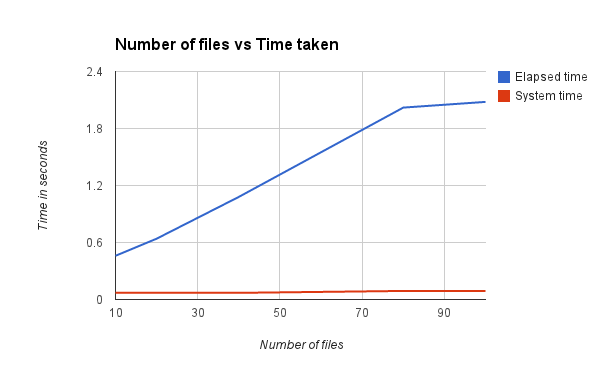
\includegraphics[width=0.8\textwidth]{20chart.png}
  \end{center}
  \caption{Execution time of calcwts for number of documents (10, 20, 40, 80, 100)}
\end{figure}

\begin{figure}[h] % Inline image example
  \begin{center}
    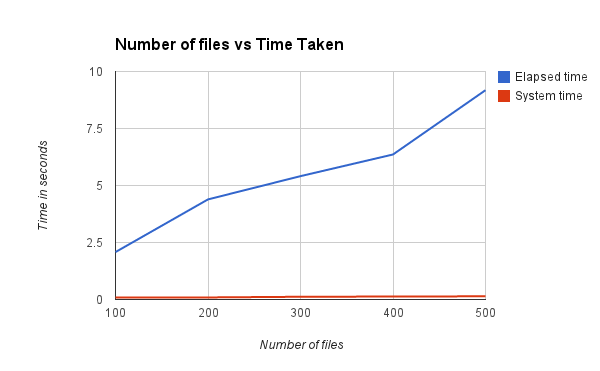
\includegraphics[width=0.8\textwidth]{100chart.png}
  \end{center}
  \caption{Execution time of calcwts for number of documents (100, 200, 300, 400, 500)}
\end{figure}

\paragraph{Profiling}

I used the line\_profiler\footnote{\url{https://pythonhosted.org/line_profiler/}} to see how much time each line of my code is taking to run. As expected tokenization and tf-idf computation takes most of the time. In the initial version of the code, profiling helped me discover bottlenecks in the program (linear time count) and I replaced it with a hashtable (constant time) to reduce the time taken exponentially (from more than 1000 seconds to just under 10 seconds).

\begin{thebibliography}{1}

\bibitem{notes} Term weighting and BM25 reference http://www.csee.umbc.edu/~nicholas/676/mir2edSlides/slides\_chap03.pdf

\bibitem{regexp} RegExp Tokenizer http://www.nltk.org/api/nltk.tokenize.html

 \bibitem{impj}Python nested dictionary http://stackoverflow.com/questions/635483/what-is-the-best-way-to-implement-nested-dictionaries-in-python
  
  \bibitem{norman} Unescape html special characters http://stackoverflow.com/questions/11405996/how-can-i-use-python-to-replace-html-escape-characters

  \bibitem{fo} Python Performance Analysis http://www.huyng.com/posts/python-performance-analysis/

  \end{thebibliography}

%%% End document
\end{document}